\documentclass{article}

\usepackage{lmodern}
\usepackage[T1]{fontenc}
\usepackage{fullpage}
\usepackage{enumitem}
\usepackage{algorithm2e}
\usepackage{filecontents}
\usepackage{listings}
\usepackage{color}
\usepackage[scaled=0.8]{DejaVuSansMono}
\usepackage{xcolor}
\usepackage[]{hyperref}
\usepackage{spverbatim}
\usepackage{todonotes}
\usepackage{amsmath}
\usepackage{tikz}
\usetikzlibrary{calc,shapes}
\lstset{escapeinside={<@}{@>}}

\DeclareUrlCommand{\url}{%
  \def\UrlFont{\color{blue}\normalfont}%      Adding a little color
  \def\UrlLeft##1\UrlRight{\underline{##1}}%  Underlining the url
}

\newcommand{\tikzmark}[1]{\tikz[overlay,remember picture] \node (#1) {};}

\lstdefinestyle{C}{language=C++,
  basicstyle=\small\ttfamily,
  keywordstyle=\color{blue}\ttfamily,
  stringstyle=\color{green}\ttfamily,
  commentstyle=\color{red}\ttfamily,
  frame=single,
  morekeywords={int64_t,include}
}

\lstdefinestyle{Bash}{language=bash,
  %keywordstyle=\color{blue},
  basicstyle=\small\ttfamily,
  deletekeywords={local},
  morekeywords={tar,mkdir,cmake,make}
}


\bibliographystyle{siam}

\newcommand{\tm}{\textsuperscript{\textregistered}}

\title{\textbf{STRUMPACK Users' Guide}}
\author{Pieter Ghysels\footnotemark[1] \\
  Xiaoye S. Li\footnotemark[1] \\
  Christopher Gorman\footnotemark[2] \\
  Gustavo Ch\'{a}vez\footnotemark[1] \\
  Fran\c{c}ois-Henry Rouet\footnotemark[3]}
\date{Version \textbf{2.2.0}, March 2018}

\begin{document}

\maketitle

\vfill

\footnotetext[1]{Lawrence Berkeley National Laboratory, Computational
  Research Division, MS 50F-1650, One Cyclotron Road, Berkeley
  CA94720. \texttt{\{pghysels,xsli,gichavez\}@lbl.gov}}
\footnotetext[2]{UC Santa Barbara. \texttt{gorman@math.ucsb.edu}}
\footnotetext[3]{Livermore Software Technology
  Corporation. \texttt{fhrouet@lstc.com}}

\pagebreak

\tableofcontents

\pagebreak
\section{STRUMPACK Overview}
STRUMPACK -- STRUctured Matrix PACKage -- is a C\texttt{++} library
% for computations with sparse and dense matrices. It uses so-called
for computations with dense and sparse matrices. It uses so-called
\emph{structured matrices}, i.e., matrices that exhibit some kind of
% low-rank property, in particular, Hierarchically Semi-Separable
low-rank property, in this case with Hierarchically Semi-Separable
matrices (HSS), to speed up linear algebra operations.  This version
of STRUMPACK unifies two main components that were separate in
previous versions: a package for dense matrix computations
(\textbf{STRUMPACK-dense}) and a package (\textbf{STRUMPACK-sparse})
for sparse linear systems. The algorithms for solving dense linear
systems are described in~\cite{rouet2014distributed} while the
algorithms for solving sparse linear systems are described
in~\cite{ghysels2015sparse,ghysels2017sparse}. STRUMPACK can be used
as a general algebraic sparse direct solver (based on the multifrontal
factorization method), or as an efficient preconditioner for sparse
matrices obtained by discretization of partial differential
equations. Included in STRUMPACK are also the GMRES and BiCGStab
iterative Krylov solvers, that use the approximate, HSS-accelerated,
sparse solver as a preconditioner for the efficient solution of sparse
linear systems.

The STRUMPACK project started at the Lawrence Berkeley National
Laboratory in 2014 and is supported by the FASTMath SciDAC Institute
funded by the Department of Energy and by the Exascale Computing
Project (17-SC-20-SC), a collaborative effort of the U.S. Department
of Energy Office of Science and the National Nuclear Security
Administration.

\noindent Check the STRUMPACK website for more information and for the
latest code:
\begin{quote}
  \url{http://portal.nersc.gov/project/sparse/strumpack/}
\end{quote}


\section{Installation and Requirements}\label{sec::installation}
The STRUMPACK package uses the CMake build system (CMake version >=
2.8). The recommended way of building the STRUMPACK library is as
follows:
\begin{lstlisting}[style=bash]
  > tar -xvzf strumpack-x.y.z.tar.gz
  > cd strumpack-x.y.x
  > mkdir build
  > cd build
  > cmake <@\textcolor{blue}{../}@> -DCMAKE_BUILD_TYPE=<@\textcolor{blue}{Release}@> \
      -DCMAKE_INSTALL_PREFIX=<@\textcolor{blue}{/path/to/install}@> \
      -DCMAKE_CXX_COMPILER=<@\textcolor{blue}{<C++ compiler>}@> \                           # this and below are optional,
      -DCMAKE_C_COMPILER=<@\textcolor{blue}{<C compiler>}@> \                               # CMake will try to autodetect
      -DCMAKE_Fortran_COMPILER=<@\textcolor{blue}{<Fortran77 compiler>}@> \
      -DSCALAPACK_LIBRARIES=<@\textcolor{blue}{"/path/to/scalapack/libscalapack.a;/path/to/blacs/libblacs.a"}@> \
      -DMETIS_INCLUDES=<@\textcolor{blue}{/path/to/metis/incluce}@> \
      -DMETIS_LIBRARIES=<@\textcolor{blue}{/path/to/metis/libmetis.a}@> \
      -DSTRUMPACK_USE_PARMETIS=ON \                                   # optional
      -DPARMETIS_INCLUDES=<@\textcolor{blue}{/path/to/parmetis/include}@> \
      -DPARMETIS_LIBRARIES=<@\textcolor{blue}{/path/to/parmetis/libparmetis.a}@> \
      -DSTRUMPACK_USE_SCOTCH=ON \                                     # optional
      -DSCOTCH_INCLUDES=<@\textcolor{blue}{/path/to/scotch/include}@> \
      -DSCOTCH_LIBRARIES=<@\textcolor{blue}{"/path/to/ptscotch/libscotch.a;...libscotcherr.a;...libptscotch.a;...libptscotcherr.a"}@>
  > make
  > make test   # optional, takes a while
  > make install
\end{lstlisting}
%% doxygen is not up to date!
%%  > make doc        # optional, needs doxygen
The above will only work if you have the following dependencies, and
CMake can find them:
\begin{itemize}
\item \textbf{C\texttt{++}11}, \textbf{C} and \textbf{FORTRAN77}
  compilers. CMake looks for these compilers in the standard
  locations, if they are installed elsewhere, you can specify them as
  follows:
  \begin{lstlisting}[style=Bash]
    > cmake <@\textcolor{blue}{../}@> -DCMAKE_BUILD_TYPE=<@\textcolor{blue}{Release}@>     \
           -DCMAKE_CXX_COMPILER=<@\textcolor{blue}{g++}@>            \
           -DCMAKE_C_COMPILER=<@\textcolor{blue}{gcc}@>              \
           -DCMAKE_Fortran_COMPILER=<@\textcolor{blue}{gfortran}@>
  \end{lstlisting}
\item \textbf{MPI} (Message Passing Interface) library.  You should
  not need to manually specify the MPI compiler wrappers.  CMake will
  look for MPI options and libraries and set the appropriate compiler
  and linker flags.
\item \textbf{OpenMP v4.5} support is required in the C\texttt{++}
  compiler to use the shared-memory parallelism in the code. OpenMP
  support can be disabled by adding the CMake option
  \begin{lstlisting}[style=Bash]
    -DSTRUMPACK_USE_OPENMP=OFF
  \end{lstlisting}
  OpenMP v3.1 introduces task parallelism, which is used extensively
  throughout the code. OpenMP v4.5 added the taskloop construct. CMake
  will check whether your compiler supports OpenMP and sets the
  appropriate compiler and linker flags.
\item \textbf{BLAS, LAPACK and ScaLAPACK} libraries. For performance
  it is crucial to use optimized BLAS/LAPACK libraries like for
  instance Intel\tm{} MKL, AMD\tm{} ACML, Cray\tm{} LibSci or
  OpenBLAS. The default versions of the Intel\tm{} MKL and Cray\tm{}
  LibSci BLAS libraries will use multithreaded kernels, unless when
  they are called from within an OpenMP parallel region, in which case
  they run sequentially. This is the behavior STRUMPACK relies upon to
  achieve good performance when running in MPI+OpenMP hybrid
  mode. ScaLAPACK depends on the BLACS communication library and on
  PBLAS (parallel BLAS), both of which are typically included with the
  ScaLAPACK installation (from ScaLAPACK 2.0.2, the blacs library is
  included in the ScaLAPACK library file). If CMake cannot locate
  these libraries, you can specify their path by setting the
  environment variable
  \lstinline[style=Bash]!$SCALAPACKDIR! or by specifying the libraries
  manually:
  \begin{lstlisting}[style=Bash]
    > cmake <@\textcolor{blue}{../}@> -DCMAKE_BUILD_TYPE=<@\textcolor{blue}{Release}@> \
       -DSCALAPACK_LIBRARIES=<@\textcolor{blue}{"/path/to/scalapack/libscalapack.a;/path/to/blacs/libblacs.a"}@>
  \end{lstlisting}
  Or one can also directly modify the linker flags to add the
  ScaLAPACK and BLACS libraries:
  \begin{lstlisting}[style=Bash]
    > cmake <@\textcolor{blue}{../}@> -DCMAKE_BUILD_TYPE=<@\textcolor{blue}{Release}@> \
       -DCMAKE_EXE_LINKER_FLAGS=<@\textcolor{blue}{"-L/usr/lib64/mpich/lib/ -lscalapack -lmpiblacs"}@>
  \end{lstlisting}
\item \textbf{METIS}
  ($\geq$ 5.1.0 \textbf{required}) for the nested dissection matrix
  reordering. Metis can be obtained from:

  \url{http://glaros.dtc.umn.edu/gkhome/metis/metis/download}.

  CMake looks for the Metis inlude files the library in the default
  locations as well as in
  \lstinline[style=Bash]!$METISDIR/include!  and
  \lstinline[style=Bash]!$METISDIR/lib!. Using the Bash shell, the
  METISDIR environment variable can be set as\\
  \lstinline[style=Bash]!export METISDIR=/usr/local/metis/!.
  Alternatively, you can specify the
  location of the header and library as follows:
  \begin{lstlisting}[style=Bash]
    > cmake <@\textcolor{blue}{../}@> -DCMAKE_BUILD_TYPE=<@\textcolor{blue}{Release}@> \
      -DMETIS_INCLUDES=<@\textcolor{blue}{/usr/local/metis/include}@> \
      -DMETIS_LIBRARIES=<@\textcolor{blue}{/usr/local/metis/lib/libmetis.a}@>
  \end{lstlisting}

\item \textbf{PARMETIS} (optional) for parallel nested
  dissection. ParMetis can be download from

  \url{http://glaros.dtc.umn.edu/gkhome/metis/parmetis/download}

  The steps to make sure CMake can find ParMetis are similar as for
  Metis. Enable with \lstinline[style=Bash]!-DSTRUMPACK_USE_PARMETIS!.
  The CMake variables are
  \lstinline[style=Bash]!$PARMETISDIR! or
  \lstinline[style=Bash]!PARMETIS_INCLUDES! and
  \lstinline[style=Bash]!PARMETIS_LIBRARIES!.

\item \textbf{SCOTCH} and \textbf{PT-SCOTCH}
  ($\geq$ 5.1.12) (optional) for matrix reordering. Scotch can be
  downloaded from:

  \url{http://www.labri.fr/perso/pelegrin/scotch/}

  Configuring CMake to find (PT-)Scotch is similar to Metis. Enable
  with \lstinline[style=Bash]!-DSTRUMPACK_USE_SCOTCH! For (PT-)Scotch
  the CMake variables are
  \lstinline[style=Bash]!$SCOTCHDIR! or
  \lstinline[style=Bash]!SCOTCH_INCLUDES! and
  \lstinline[style=Bash]!SCOTCH_LIBRARIES!. Make sure to specify all
  libraries: \lstinline[style=Bash]!libscotch!,
  \lstinline[style=Bash]!libscotcherr!,
  \lstinline[style=Bash]!libptscotch! and
  \lstinline[style=Bash]!libptscotcherr!.

\item \textbf{getopt\_long:} This is a GNU extension to the POSIX
  getopt() C library function.
\item \textbf{TCMalloc}, \textbf{TBB Malloc} or \textbf{jemalloc}:
  This is \textbf{optional}, but \textbf{recommended}, as it can lead
  to dramatic performance improvements for multithreaded code that
  performs frequent memory allocations. Link with the one of these
  libraries, e.g.:
  \begin{lstlisting}[style=Bash]
  -DCMAKE_EXE_LINKER_FLAGS=<@\textcolor{blue}{"-ltcmalloc"}@>
  \end{lstlisting}
  to replace the default memory allocator (C\texttt{++} \texttt{new})
  with a more scalable implementation. See also
  Section~\ref{sec:tips}.
\end{itemize}
The code was tested on GNU/Linux with the GNU and Intel\tm{} compilers
and the OpenBLAS, Intel\tm{} MKL\tm{} and Cray\tm{} LibSci\tm{}
numerical libraries. If you encounter issues on other platforms or
with other BLAS/LAPACK implementations, please let us know.
Successful compilation will create a
\textcolor{green}{\texttt{libstrumpack.a}} file.


\section{Algorithm}\label{sec:algo}
The algorithm used in STRUMPACK is described in detail
in~\cite{ghysels2015sparse}, and is based on the work by Jianlin
Xia~\cite{xia2013randomized}. Here we summarize the main algorithm
features. Section~\ref{sec:HSS} has more information on the low-rank
compression strategy and how to tune this to get a good preconditioner
for your specific problem. There are three main steps in the
algorithm: matrix reordering, factorization and solve.

\begin{description}
\item[Matrix reordering:] There are three distinct matrix reordering
  steps: one for stability, one to limit fill-in and one to reduce
  HSS-ranks. First, the matrix is reordered and possibly scaled for
  numerical stability by the MC64 code~\cite{duff1999design}. For many
  matrices, this reordering can safely be disabled. By default, MC64
  is used to maximize the product of the diagonal values of the
  matrix, and to scale the rows and columns of the
  matrix. Alternatively, MC64 can be used to maximize the smallest
  diagonal value or to maximize the sum of the diagonals. Next, a
  nested dissection reordering is applied to limit fill-in.  Both
  (Par)Metis and (PT-)Scotch are supported. We expose one user tunable
  parameter which controls the size of the smallest
  separators. Finally, when HSS compression is used, there is an extra
  reordering step to reduce the HSS-ranks. This reordering uses Metis
  and does not require user tuning.

\item[Factorization:] Before the actual numerical factorization, there
  is a symbolic factorization step to construct the elimination
  tree. After that, the multifrontal factorization procedure traverses
  this elimination tree from bottom (smallest separators) to top (root
  separator). With each node of the elimination tree a dense matrix is
  associated, referred to as a frontal matrix, or simply front. These
  fronts can possibly be compressed as Hierarchically Semi-Separable
  (HSS) matrices. This compression will only pay off for fronts that
  are large enough, which are typically the frontal matrices at the
  nodes in the elimination tree close to the root. Without any HSS
  compression, the solver acts as a standard multifrontal direct
  solver. HSS approximations are constructed using a randomized
  sampling algorithm.

\item[Solve:] Once the matrix is factorized, the factors can be used
  to efficiently solve a linear system of equations by doing a forward
  and a backward solve sweeps. When no HSS compression is used, this
  is a direct solver. The multifrontal solve procedure is then used
  within an iterative refinement loop, with typically only 1 or very
  few iterations. However, when the factors are compressed using HSS,
  a single multifrontal solve is only approximate and the solve is by
  default used as a preconditioner for GMRES($30$). The required
  number of GMRES iterations will depend strongly on the quality of
  the HSS approximation.
\end{description}

\section{Using STRUMPACK Sparse}\label{sec:usage}
This section gives an overview on the basic usage of the sparse
solvers in STRUMPACK.
% Additionally, we refer to the online automatically
% generated Doxygen pages at
% \begin{quote}
%   \url{http://portal.nersc.gov/project/sparse/strumpack/doxygen}
% \end{quote}
% for a complete and up-to-date documentation of the STRUMPACK API.
Many STRUMPACK options can be set from the command line. Running with
\lstinline[style=Bash]!--help! or \lstinline[style=Bash]!-h!, will
give you a list of supported run-time options.

An example \lstinline[style=Bash]!Makefile! is available in the
\lstinline[style=Bash]!examples/! directory. This
\lstinline[style=Bash]!Makefile! is generated by the
\lstinline[style=Bash]!cmake! command, see
Section~\ref{sec::installation}.

The STRUMPACK package is written in C\texttt{++}, and offers a simple
C\texttt{++} interface. See Section~\ref{sec:Cinterface} if you prefer
a C interface. STRUMPACK-sparse has three different solver classes,
all interaction happens through objects of these classes:
\begin{itemize}
\item \textbf{\lstinline[style=C]!StrumpackSparseSolver<scalar,integer=int>!}\\
  This class represents the sparse solver for a single computational
  node, optionally using OpenMP parallelism. Use this if you are
  running the code sequentially, on a (multicore) laptop or desktop or
  on a single node of a larger cluster. This class is defined in
  \lstinline[style=Bash]!StrumpackSparseSolver.hpp!, so include this
  header if you intend to use it.
\item \textbf{\lstinline[style=C]!StrumpackSparseSolverMPI<scalar,integer=int>!}\\
  This solver has (mostly) the same interface as
  \lstinline[style=C]!StrumpackSparseSolver<scalar,integer>!  but
  the numerical factorization and multifrontal solve phases run in
  parallel using MPI and ScaLAPACK. However, the inputs (sparse
  matrix, right-hand side vector) need to be available completely on
  every MPI process. The reordering phase uses Metis or Scotch (not
  ParMetis or PTScotch) and the symbolic factorization is threaded,
  but not distributed. The (multifrontal) solve is done in parallel,
  but the right-hand side vectors need to be available completely on
  every processor. Make sure to call
%  \lstinline[style=C]!MPI_Init(_thread)!  before instantiating an
  \lstinline[style=C]!MPI_Init[_thread]!  before instantiating an
  object of this class and include the header file
  \lstinline[style=Bash]!StrumpackSparseSolverMPI.hpp!. We do not
  recommend this solver, instead, use
  \lstinline[style=C]!StrumpackSparseSolverMPIDist! whenever possible.
\item
  \textbf{\lstinline[style=C]!StrumpackSparseSolverMPIDist<scalar,integer=int>!}\\
  This solver is fully distributed. The numerical factorization and
  solve as well as the symbolic factorization are distributed. The
  input is now a block-row distributed sparse matrix and a
  correspondingly distributed right-hand side. For matrix reordering,
  ParMetis or PT-Scotch are used. Include the header file
  \lstinline[style=Bash]!StrumpackSparseSolverMPIDist.hpp! and call
%  \lstinline[style=C]!MPI_Init(_thread)!. Unfortunately, there is no
  \lstinline[style=C]!MPI_Init[_thread]!. Unfortunately, there is no
  distributed version of the MC64 reordering code, so if this
  reordering (and scaling) step is enabled, the code will gather the
  distributed sparse matrix on a single node and then apply MC64
  sequentially.
\end{itemize}

The three solver classes \lstinline[style=C]!StrumpackSparseSolver!,
\lstinline[style=C]!StrumpackSparseSolverMPI! and\\
\lstinline[style=C]!StrumpackSparseSolverMPIDist! depend on two
template parameters \lstinline[style=C]!<scalar,integer>!: the type of
a scalar and an integer type. The scalar type can be
\lstinline[style=C]!float!, \lstinline[style=C]!double!,
\lstinline[style=C]!std::complex<float>! or
\lstinline[style=C]!std::complex<double>!. It is recommended to first
try to simply use the default \lstinline[style=C]!integer=int! type,
unless you run into 32 bit integer overflow problems. In that case one
can switch to for instance \lstinline[style=C]!int64_t! (a signed
integer type).

\subsection{StrumpackSparseSolver Example}
The following shows the typical way to use a (sequential or
multithreaded) STRUMPACK sparse solver:
\begin{lstlisting}[style=C]
#include "StrumpackSparseSolver.hpp"
using namespace strumpack;  // all strumpack code is in the strumpack namespace,

int main(int argc, char* argv[]) {
  int N = ...;                // construct an NxN CSR matrix with nnz nonzeros
  int* row_ptr = ...;         // N+1 integers
  int* col_ind = ...;         // nnz integers
  double* val = ...;          // nnz scalars
  double* x = new double[N];  // will hold the solution vector
  double* b = ...;            // set a right-hand side b

  StrumpackSparseSolver<double> sp;               // create solver object
  sp.options().set_rel_tol(1e-10);                // set options
  sp.options().set_gmres_restart(10);             // ...
  sp.options().enable_HSS();                      // enable HSS compression, see section <@\ref{sec:HSS}@>
  sp.options().set_from_command_line(argc, argv); // parse command line options
  sp.set_csr_matrix(N, row_ptr, col_ind, val);    // set the matrix (copy)
  sp.reorder();                                   // reorder matrix
  sp.factor();                                    // numerical factorization
  sp.solve(b, x);                                 // solve Ax=b
  ... // check residual/error and cleanup
}
\end{lstlisting}
The main steps are: create solver object, set options (parse options
from the command line), set matrix, reorder, factor and finally
solve. The matrix should be in the Compressed Sparse Row (CSR) format,
also called Yale format, with $0$ based indices. Figure~\ref{fig::csr}
illustrates the CSR format. In the basic scenario, it is not necessary
to explicitly call \lstinline[style=C]!reorder!  and
\lstinline[style=C]!factor!, since trying to solve with a
\lstinline[style=C]!StrumpackSparseSolver! object that is not factored
yet, will internally call the \lstinline[style=C]!factor! routine,
which will call \lstinline[style=C]!reorder! if necessary.

\begin{figure}
  \begin{center}
    \begin{minipage}{.39\textwidth}
      \[
        A = \begin{bmatrix}
          8.2 & 0.1 & & & 3.1 \\
          0 &  & -4.8 \\
          6.2 & 1.1 &  & 2.6 \\
          & & -1.0 &  &  \\
          & & & 99.9 & 4.0
        \end{bmatrix}
      \]
    \end{minipage}
    \begin{minipage}{.59\textwidth}
      \vspace{.4cm}
      \begin{align*}
        \texttt{row\_ptr} &= [\tikzmark{a1}0, \, \tikzmark{a2}3, \, \tikzmark{a3}5, \, \tikzmark{a4}8, \, \tikzmark{a5}9, \, 11 ] \\
        \\
        \texttt{col\_ind} &= [ \tikzmark{b1}0,   \, 1,   \, 4   \, | \, 0\tikzmark{b2}, \, 2    \,| \, 0\tikzmark{b3},   \, 1,   \, 3
                          \,| \, 2\tikzmark{b4}    \,| \, 3\tikzmark{b5},    \, 4   ] \\
        \texttt{values} &= [ 8.2, \, 0.1, \, 3.1 \, | \, 0, \, -4.8 \,| \, 6.2, \, 1.1, \, 2.6 \,| \, -1.0 \,| \, 99.9, \, 4.0 ] \\
        \begin{tikzpicture}[overlay,remember picture,-latex,shorten >=5pt,shorten <=5pt,out=70,in=130]
          \draw (a1.south)+(0,0.2) -- (b1.north);
          \draw (a2.south)+(0,0.15) -- (b2.north);
          \draw (a3.south)+(0,0.15) -- (b3.north);
          \draw (a4.south)+(0,0.15) -- (b4.north);
          \draw (a5.south)+(0,0.15) -- (b5.north);
        \end{tikzpicture}
      \end{align*}
    \end{minipage}
    \vspace{-.4cm}
  \end{center}
  \caption{Illustration of a small $5 \times 5$ sparse matrix with
    $11$ nonzeros and its Compressed Sparse Row (CSR) or Yale format
    representation. We always use $0$-based indexing! Let $N=5$ denote
    the number of rows. The \texttt{row\_ptr} array has $N+1$
    elements, with element $i$ denoting the start of row $i$ in the
    \texttt{col\_ind} and \texttt{values} arrays. Element
    \texttt{row\_ptr[N] = nnz}, i.e., the total number of nonzero
    elements in the matrix. The \texttt{values} array holds the actual
    matrix values, ordered by row. The corresponding elements in
    \texttt{col\_ind} give the column indices for each nonzero. There
    can be explicit zero elements in the matrix. The nonzero values
    and corresponding column indices need not be sorted by column
    (within a row).}
  \label{fig::csr}
\end{figure}


The above code should be linked with
\lstinline[style=Bash]!-lstrumpack! and with the Metis,
ParMetis, Scotch, PT-Scotch, BLAS, LAPACK, and ScaLAPACK libraries.\\

\subsection{StrumpackSparseSolverMPI Example}
Usage of the
\lstinline[style=C]!StrumpackSparseSolverMPI<scalar,integer=int>!
solver is very similar:
\begin{lstlisting}[style=C]
#include "StrumpackSparseSolverMPI.hpp"
using namespace strumpack;

int main(int argc, char* argv[]) {
  int thread_level, rank;
  // StrumpackSparseSolverMPI uses OpenMP so we should ask for MPI_THREAD_FUNNELED at least
  MPI_Init_thread(&argc, &argv, MPI_THREAD_FUNNELED, &thread_level);
  MPI_Comm_rank(MPI_COMM_WORLD, &rank);
  if (thread_level != MPI_THREAD_FUNNELED && rank == 0)
    std::cout << "MPI implementation does not support MPI_THREAD_FUNNELED" << std::endl;

  {
    // define the same CSR matrix as for StrumpackSparseSolver
    int N = ...;                // construct an NxN CSR matrix with nnz nonzeros
    int* row_ptr = ...;         // N+1 integers
    int* col_ind = ...;         // nnz integers
    double* val = ...;          // nnz scalars
    // allocate entire solution and right-hand side vectors on each MPI process
    double* x = new double[N];  // will hold the solution vector
    double* b = ...;            // set a right-hand side b

    // construct solver and specify the MPI communicator
    StrumpackSparseSolverMPI<double> sp(MPI_COMM_WORLD);
    sp.options().set_mc64job(0);
    sp.options().set_from_command_line(argc, argv);
    sp.set_csr_matrix(N, row_ptr, col_ind, val);
    sp.solve(b, x);
    ... // check residual/error, cleanup
  }
  Cblacs_exit(1);
  MPI_Finalize();
}
\end{lstlisting}
The only difference here is the use of
\lstinline[style=C]!StrumpackSparseSolverMPI! instead of
\lstinline[style=C]!StrumpackSparseSolver! and the calls to
\lstinline[style=C]!MPI_Init_thread!, \lstinline[style=C]!Cblacs_exit!
and \lstinline[style=C]!MPI_Finalize!.\\


\subsection{StrumpackSparseSolverMPIDist Example}
Finally, we illustrate the usage of
\lstinline[style=C]!StrumpackSparseSolverMPIDist<scalar,integer=int>!
solver. This interface takes a block-row distributed compressed sparse
row matrix as input. This matrix format is illustrated in
Figure~\ref{fig::block-row-csr}.
\begin{lstlisting}[style=C]
#include "StrumpackSparseSolverMPI.hpp"
using namespace strumpack;

int main(int argc, char* argv[]) {
  int thread_level, rank, P;
  MPI_Init_thread(&argc, &argv, MPI_THREAD_FUNNELED, &thread_level);
  MPI_Comm_rank(MPI_COMM_WORLD, &rank);
  MPI_Comm_size(MPI_COMM_WORLD, &P);
  {
    // define a block-row distributed CSR matrix
    int* dist     = new int[P];
    // set dist such that processor p owns rows [dist[p], dist[p+1]) of the sparse matrix
    for (int p=0; p<P; p++) dist[p] = .. ;
    // local_n is the number of rows of the input matrix assigned to me
    int local_n   = dist[rank+1] - dist[rank];
    int* row_ptr  = new int[local_n+1];
    .. // set the sparse matrix row pointers in row_ptr
    int local_nnz = row_ptr[local_n+1] - row_ptr[0];
    int* col_ind  = new int[local_nnz];
    .. // set the sparse matrix column indices in col_ind
    double* val   = new double[local_nnz];
    .. // set the matrix nonzero value in val
    double* x     = new double[local_n];        // local part of solution
    double* b     = new double[local_n];        // local part of rhs
    for (int i=0; i<local_n; i++) b[i] = ..;    // set the rhs

    StrumpackSparseSolverMPIDist<double> sp(MPI_COMM_WORLD);
    sp.options().set_reordering_method(ReorderingStrategy::PARMETIS);
    sp.options().set_from_command_line(argc, argv);
    sp.set_distributed_csr_matrix(local_n, row_ptr, col_ind, val, dist);
    sp.solve(b, x);
    ... // check residual/error, cleanup
  }
  Cblacs_exit(1);
  MPI_Finalize();
}
\end{lstlisting}

\begin{figure}
  \begin{center}
    \begin{equation*}
      A = \begin{bmatrix}
        8.2 & 0.1 & & & 3.1 \\
        \hline
        0 &  & -4.8 \\
        6.2 & 1.1 &  & 2.6 \\
        \hline
        & & -1.0 &  &  \\
        & & & 99.9 & 4.0
      \end{bmatrix}
      \begin{matrix}  P_0 \\ \vspace{-.2cm} \\ P_1 \\  \\ P_2 \vspace{.2cm}\end{matrix}
    \end{equation*}
    \begin{equation*}
      \texttt{dist} = [ 0, \, 1, \, 3, \, 5 ]
      \vspace{-.5cm}
    \end{equation*}
    \begin{minipage}{.3\textwidth}
      \begin{align*}
        P_0 \\
        \texttt{row\_ptr} &= [ 0, \, 3 ] \\
        \texttt{col\_ind} &= [ 0, \, 1,   \, 4 ] \\
        \texttt{values}   &= [ 8.2, \, 0.1, \, 3.1 ]
      \end{align*}
    \end{minipage}
    \begin{minipage}{.3\textwidth}
      \begin{align*}
        P_1 \\
        \texttt{row\_ptr} &= [ 0, \, 2, \, 5 ] \\
        \texttt{col\_ind} &= [ 0, \, 2  \,| \, 0, \, 1, \, 3 ] \\
        \texttt{values}   &= [ 0, \, -4.8 \,| \, 6.2, \, 1.1, \, 2.6 ]
      \end{align*}
    \end{minipage}
    \begin{minipage}{.3\textwidth}
      \begin{align*}
        P_2 \\
        \texttt{row\_ptr} &= [ 0, \, 1, \, 3 ] \\
        \texttt{col\_ind} &= [ 2  \,| \, 3, \, 4 ] \\
        \texttt{values} &= [ -1.0 \,| \, 99.9, \, 4.0 ]
      \end{align*}
    \end{minipage}
  \end{center}
  \caption{Illustration of a small $5 \times 5$ sparse matrix with
    $11$ nonzeros and its block-row distributed compressed sparse row
    representation. We always use $0$-based indexing! Process $P_0$
    owns row $0$, process $P_1$ has rows $1$ and $2$ and process $P_2$
    has rows $3$ and $4$. This distribution of rows over the processes
    is represented by the \texttt{dist} array. Process p owns rows
    \texttt{[dist[p],dist[p+1])}. If $N=5$ is the number of rows in
    the entire matrix and P is the total number of processes, then
    \texttt{dist[P]=N}. The (same) \texttt{dist} array is stored on
    every process. Each process holds a CSR representation of only its
    local rows of the matrix, see Figure~\ref{fig::csr}.}
  \label{fig::block-row-csr}
\end{figure}

\subsection{Initializing the Solver Object}\label{sec:initsolver}
Let
\begin{lstlisting}[style=C]
  typedef strumpack::StrumpackSparseSolver<scalar,integer> Sp;
  typedef strumpack::StrumpackSparseSolverMPI<scalar,integer> SpMPI;
  typedef strumpack::StrumpackSparseSolverMPIDist<scalar,integer> SpMPIDist;
\end{lstlisting}
Each of the solver classes has two constructors:
\begin{lstlisting}[style=C]
  Sp::StrumpackSparseSolver(bool verbose=true, bool root=true);
  Sp::StrumpackSparseSolver(int argc, char* argv[], bool verbose=true, bool root=true);
\end{lstlisting}

\begin{lstlisting}[style=C]
  SpMPI::StrumpackSparseSolverMPIDist(MPI_Comm comm, bool verbose=true);
  SpMPI::StrumpackSparseSolverMPIDist(MPI_Comm comm, int argc, char* argv[], bool verbose=true);
\end{lstlisting}

\begin{lstlisting}[style=C]
  SpMPIDist::StrumpackSparseSolverMPIDist(MPI_Comm comm, bool verbose=true);
  SpMPIDist::StrumpackSparseSolverMPIDist(MPI_Comm comm, int argc, char* argv[], bool verbose=true);
\end{lstlisting}
where \lstinline[style=C]!argc! and \lstinline[style=C]!argv! contain
the command line options and the \lstinline[style=C]!verbose! option
can be set to \lstinline[style=C]!false! to suppress output of the
solver. Note that since \lstinline[style=C]!SpMPIDist! is a subclass
of \lstinline[style=C]!SpMPI!, which is a subclass of
\lstinline[style=C]!Sp!, all public members of Sp are also members of
\lstinline[style=C]!SpMPI! and \lstinline[style=C]!SpMPIDist!. The
public interface to the \lstinline[style=C]!SpMPI! class is exactly
the same as that for the \lstinline[style=C]!Sp! class.

\subsection{Sparse Matrix Format}
The sparse matrix should be specified in compressed sparse row
format~\cite{saad2003iterative}:
\begin{lstlisting}[style=C]
  void Sp::set_csr_matrix(int N, int* row_ptr, int* col_ind, scalar* values,
                          bool symmetric_pattern=false);
\end{lstlisting}
% void Sp::set_csc_matrix(int N, int* col_ptr, int* row_ind, scalar* values,
% bool symmetric_pattern=false);
Internally, the matrix is copied, so it will not be modified. Previous
versions of STRUMPACK also supported the CSC format, but this is now
deprecated. If the sparsity pattern of the matrix is symmetric (the
values do not have to be symmetric), then you can set
\lstinline[style=C]!symmetric_pattern=true!. This saves some work in
the setup phase of the solver.

For the \lstinline[style=C]!SpMPIDist! solver the input is a block-row
distributed compressed sparse row matrix (as illustrated in the
example above):
\begin{lstlisting}[style=C]
  void SpMPIDist::set_distributed_csr_matrix
         (integer local_rows, integer* row_ptr, integer* col_ind,
          scalar* values, integer* dist, bool symmetric_pattern=false);
\end{lstlisting}
Alternatively, you can also specify a sequential CSR matrix to the
\lstinline[style=C]!SpMPIDist! solver:
\begin{lstlisting}[style=C]
  void SpMPIDist::set_csr_matrix
         (integer N, integer* row_ptr, integer* col_ind,
          scalar* values, bool symmetric_pattern=false);
\end{lstlisting}
For this routine, the matrix only needs to be specified completely on
the root process. Other processes can pass \lstinline[style=C]!NULL!
for the arrays.

\subsection{Setting and Parsing Options}
The solver class has an object of type
\lstinline[style=C]!SPOptions<scalar>!, which can be accessed through:
\begin{lstlisting}[style=C]
  SPOptions<scalar>& Sp::options();
\end{lstlisting}
The \lstinline[style=C]!SPOptions<scalar>! class is defined in
\lstinline[style=Bash]!SPOptions.hpp!. The complete public interface
for the \lstinline[style=C]!SPOptions<scalar>! class is given in
Section~\ref{sec:SPOptions}. The following subsections describe some
of the options available from \lstinline[style=C]!SPOptions<scalar>!
in more detail.

% Once the solver object is created, options can be set on
% it.  Then, calling the function
% \lstinline[style=C]!StrumpackSparseSolver::set_from_options()!  will
% parse the command line options from \lstinline[style=C]!argv!,
% possibly overwriting any options defined on the
% \lstinline[style=C]!StrumpackSparseSolver! before this point. When one
% of the options is \lstinline[style=Bash]!--help! or
% \lstinline[style=Bash]!-h!, a list of all possible options is printed
% and the code exits.

\subsection{Reordering}
There are three types of matrix reordering: for numerical stability,
to reduce fill-in and to reduce the HSS-ranks. These reorderings are
all performed when calling
\begin{lstlisting}[style=C]
  ReturnCode Sp::reorder();
\end{lstlisting}
The return value is of type \lstinline[style=C]!ReturnCode!  (defined
in \lstinline[style=Bash]!strumpack_parameters.hpp!) and can be
\begin{lstlisting}[style=C]
  enum class ReturnCode {
    SUCCESS,          /*!< Operation completed successfully. */
    MATRIX_NOT_SET,   /*!< The input matrix was not set.     */
    REORDERING_ERROR  /*!< The matrix reordering failed.     */
  };
\end{lstlisting}

\subsubsection{Reordering for numerical stability}\label{sec::mc64}
The reordering for numerical stability is performed using the MC64
code. For many matrices, this reordering is not necessary and can
safely be disabled! MC64 supports 5 different modes
{\small \begin{itemize}
\item[\textbf{0:}] no reordering for stability, this disables MC64
\item[\textbf{1:}] currently not supported
\item[\textbf{2:}] maximize the smallest diagonal value
\item[\textbf{3:}] maximize the smallest diagonal value, different strategy
\item[\textbf{4:}] maximize sum of diagonal values
\item[\textbf{5:}] maximize product of diagonal values and apply row and column scaling
\end{itemize}}
which can be selected via
\begin{lstlisting}[style=C]
  void SPOptions::set_mc64job(int job);
  void SPOptions::set_mc64job(MC64Job job);
  int SPOptions::mc64job() const;
\end{lstlisting}
where \lstinline[style=C]!mc64()! queries the currently selected
strategy (the default is \textbf{5:} maximum product of diagonal
values plus row and column scaling). Instead of entering a number, you
can specify one of the enumerations in \lstinline[style=C]!MC64Job!:
\begin{lstlisting}[style=C]
  enum class MC64Job {
    NONE,                         /*!< Don't do anything                                              */
    MAX_CARDINALITY,              /*!< Maximum cardinality                                            */
    MAX_SMALLEST_DIAGONAL,        /*!< Maximum smallest diagonal value                                */
    MAX_SMALLEST_DIAGONAL_2,      /*!< Same as MAX_SMALLEST_DIAGONAL, different algorithm             */
    MAX_DIAGONAL_SUM,             /*!< Maximum sum of diagonal values                                 */
    MAX_DIAGONAL_PRODUCT_SCALING  /*!< Maximum product of diagonal values and row and column scaling  */
  };
\end{lstlisting}
The command line option
\begin{lstlisting}[style=Bash]
  --sp_mc64job [0-5]
\end{lstlisting}
can also be used.

\subsubsection{Nested dissection reordering}\label{sec:ND}
The STRUMPACK sparse solver supports both (Par)Metis and (PT-)Scotch
for the matrix reordering. The following functions can set the
preferred method or check the currently selected method:
\begin{lstlisting}[style=C]
  void SPOptions::set_reordering_method(ReorderingStrategy m);
  ReorderingStrategy SPOptions::reordering_method() const;
\end{lstlisting}
The options for
\lstinline[style=C]!MatrixReorderingStrategy! are
\begin{lstlisting}[style=C]
  enum class ReorderingStrategy {
    NATURAL,    /*!< Do not reorder the system                      */
    METIS,      /*!< Use Metis nested-dissection reordering         */
    PARMETIS,   /*!< Use ParMetis nested-dissection reordering      */
    SCOTCH,     /*!< Use Scotch nested-dissection reordering        */
    PTSCOTCH,   /*!< Use PT-Scotch nested-dissection reordering     */
    RCM,        /*!< Use RCM reordering                             */
    GEOMETRIC   /*!< A simple geometric nested dissection code that
                  only works for regular meshes. (see Sp::reorder)  */
  };
\end{lstlisting}
When the solver is an object of \lstinline[style=C]!Sp!,
\lstinline[style=C]!PARMETIS! or \lstinline[style=C]!PTSCOTCH! are not
supported.  When the solver is parallel, either an
\lstinline[style=C]!SpMPI! or \lstinline[style=C]!SpMPIDist! object,
and \lstinline[style=C]!METIS!, \lstinline[style=C]!SCOTCH! or
\lstinline[style=C]!RCM! are chosen, then the graph of the complete
matrix will be gathered onto the root process and the root process
will call the (sequential) Metis, Scotch or RCM reordering
routine. For large graphs this might fail due to insufficient memory.

The \lstinline[style=C]!GEOMETRIC! option is only allowed for regular
grids. In this case, the dimensions of the grid should be specified in
the function
\begin{lstlisting}[style=C]
  ReturnCode Sp::reorder(int nx=1, int ny=1, int nz=1);
\end{lstlisting}
For instance for a regular 2d $2000 \times 4000$ grid, you can call
this as \lstinline[style=C]!sp.reorder(2000, 4000)!. In the general
algebraic case, the grid dimensions don't have to be provided. The
reordering method can also be specified via the command line option
\begin{lstlisting}[style=Bash]
  --sp_reordering_method [metis|parmetis|scotch|ptscotch|geometric|rcm]
\end{lstlisting}


\subsection{Factorization}
Compute the factorization by calling
\begin{lstlisting}[style=C]
  ReturnCode Sp::factor();
\end{lstlisting}
where the possible return values are the same as for
\lstinline[style=C]!Sp::reorder()!.  If
\lstinline[style=C]!Sp::reorder()! was not called already, it is
called automatically. When HSS compression is not enabled, this will
compute an exact LU factorization of the (permuted) sparse input
matrix. If HSS compression is enabled (with
\lstinline[style=C]!SPOptions::enable_HSS()! or
\lstinline[style=Bash]!--sp_enable_HSS!, see Section~\ref{sec:HSS}),
the factorization is only approximate.

\subsection{Solve}\label{subsec:use_solve}
Solve the linear system $Ax=b$ by calling
\begin{lstlisting}[style=C]
  ReturnCode Sp::solve(scalar* b, scalar* x, bool use_initial_guess=false);
\end{lstlisting}
By default (\lstinline[style=C]!bool use_initial_guess=false!) the
input in \lstinline[style=C]!x! is ignored. If
\lstinline[style=C]!bool use_initial_guess=true!,
\lstinline[style=C]!x! is used as initial guess for the iterative
solver (if an iterative solver is used, for instance iterative
refinement or GMRES). If the \lstinline[style=C]!Sp::factor()! was not
called, it is called automatically. The return values are the same as
for \lstinline[style=C]!Sp::reorder()!.

The iterative solver can be chosen through:
\begin{lstlisting}[style=C]
  void SPOptions::set_Krylov_solver(KrylovSolver s);
\end{lstlisting}
where \lstinline[style=C]!KrylovSolver! can take the following values:
\begin{lstlisting}[style=C]
  enum class KrylovSolver {
    AUTO,          /*!< Use iterative refinement if no HSS compression is used, otherwise PGMRES.        */
    DIRECT,        /*!< No outer iterative solver, just a single application of the multifrontal solver. */
    REFINE,        /*!< Iterative refinement.                                                            */
    PREC_GMRES,    /*!< Preconditioned GMRES. The preconditioner is the (approx) multifrontal solver.    */
    GMRES,         /*!< UN-preconditioned GMRES. (for testing mainly)                                    */
    PREC_BICGSTAB, /*!< Preconditioned BiCGStab. The preconditioner is the (approx) multifrontal solver. */
    BICGSTAB       /*!< UN-preconditioned BiCGStab. (for testing mainly)                                 */
  };
\end{lstlisting}
with \lstinline[style=C]!KrylovSolver::AUTO! being the default value.
The \lstinline[style=C]!KrylovSolver::AUTO! setting will use iterative
refinement when HSS compression is not enabled, and preconditioned
GMRES when HSS compression is enabled, see Section~\ref{sec:HSS}.  To
use the solver as a preconditioner, or a single (approximate) solve,
set the solver to \lstinline[style=C]!KrylovSolver::DIRECT!. When
calling \lstinline[style=C]!SpMPIDist::solve!, the right-hand side and
solution vectors should only point to the local parts!


\subsection{All Options for the Sparse Solver}
The HSS specific options are stored in an object of type
\lstinline[style=C]!HSSOptions<scalar>!, inside the
\lstinline[style=C]!SPOptions! object. These options are described in
Section~\ref{sec:HSS}.

\subsubsection{\lstinline[style=C]!SPOptions<scalar>! Interface}
\label{sec:SPOptions}
The complete public interface to the options class is as follows, wher
the \lstinline[style=C]!real! type is the real part of a scalar, i.e.,
\lstinline[style=C]!decltype(std::real(scalar(0)))!.
\begin{lstlisting}[style=C]
  template<typename scalar> class SPOptions {
  public:
    SPOptions();
    SPOptions(int argc, char* argv[]);

    /* print statistics?                                             */
    void set_verbose(bool verbose);                       bool verbose() const;
    /* maximum iterations in iterative solver                        */
    void set_maxit(int maxit);                            int maxit() const;
    /* relative residual stopping criterion for iterative solver     */
    void set_rel_tol(real rel_tol);                       real rel_tol() const;
    /* absolute residual stopping criterion for iterative solver     */
    void set_abs_tol(real abs_tol);                       real abs_tol() const;
    /* type of iterative solver to use, see section <@\ref{subsec:use_solve}@>              */
    void set_Krylov_solver(KrylovSolver s);               KrylovSolver Krylov_solver() const;
    /* GMRES restart                                                 */
    void set_gmres_restart(int m);                        int gmres_restart() const;
    /* type of Gram-Schmidt used in GMRES                            */
    void set_GramSchmidt_type(GramSchmidtType t);         GramSchmidtType GramSchmidt_type() const;
    /* nested-dissection code, see section <@\ref{sec:ND}@>                     */
    void set_reordering_method(ReorderingStrategy m);     ReorderingStrategy reordering_method() const;
    /* stop nested-dissection when domains are smaller than nd_param */
    void set_nd_param(int nd_param);                      int nd_param() const;
    /* use the internal (undocumented) metis routine METIS_NodeNDP   */
    void enable_METIS_NodeNDP();                          bool use_METIS_NodeNDP() const;
    /* do not use METIS_NodeNDP, use METIS_NodeND instead            */
    void disable_METIS_NodeNDP();
    /* use METIS_NodeND instead of METIS_NodeDNP                     */
    void enable_METIS_NodeND();                           bool use_METIS_NodeND() const;
    /* do not use METIS_NodeND, use METIS_NodeNDP instead            */
    void disable_METIS_NodeND();
    /* build the supernodal tree using the MUMPS_SYMQAMD code        */
    void enable_MUMPS_SYMQAMD();                          bool use_MUMPS_SYMQAMD() const;
    /* do not use MUMPS_SYMQAMD, use fundamental supernodes          */
    void disable_MUMPS_SYMQAMD();
    /* when using MUMPS_SYMQAMS, enable aggressive amalgamation      */
    void enable_agg_amalg();                              bool use_agg_amalg() const;
    /* when using MUMPS_SYMQAMS, disable aggressive amalgamation      */
    void disable_agg_amalg();
    /* set the job to be used for static pivoting, see section <@\ref{sec::mc64}@>  */
    void set_mc64job(int job);                            int mc64job() const;
    void set_mc64job(MC64Job job);
    /* not used at the moment                                         */
    void enable_assembly_tree_log();                      bool log_assembly_tree() const;
    void disable_assembly_tree_log();

    /* enable HSS compression, see section <@\ref{sec:HSS}@>                          */
    void enable_HSS();                                    bool use_HSS() const;
    /* disable HSS compression                                        */
    void disable_HSS();
    /* set the minimum size of a separator for HSS compression        */
    void set_HSS_min_sep_size(int s);                     int HSS_min_sep_size() const;

    /* set level to 1 to enable length 2 connections in the separator
     * before computing separator reordering to reduce HSS ranks.
     * Set to to disable length 2 connections.                        */
    void set_separator_ordering_level(int l);             int separator_ordering_level() const;

    /* best not to touch this                                         */
    void enable_indirect_sampling();
    void disable_indirect_sampling();                     bool indirect_sampling() const;

    void enable_replace_tiny_pivots();                    bool replace_tiny_pivots() const;
    void disable_replace_tiny_pivots(;

    /* get the HSS specific options, see section <@\ref{sec:HSS}@>.                   */
    const HSS::HSSOptions<scalar>& HSS_options() const;
    HSS::HSSOptions<scalar>& HSS_options();

    /* parse the options in argc/argv set in the constructor          */
    void set_from_command_line();
    /* parse the options in argc/argv                                 */
    void set_from_command_line(int argc, char* argv[]);
    /* print out message listing all command line options             */
    void describe_options() const;
  };
\end{lstlisting}
% /* set the minimum size of a front for HSS compression            */
% void set_HSS_min_front_size(int s);                   int HSS_min_front_size() const;
This uses the following (scoped) enumeration for the Gram-Schmidt type
used in GMRES:
\begin{lstlisting}[style=C]
  enum class GramSchmidtType {
    CLASSICAL,   /*!< Classical Gram-Schmidt is faster, more scalable.   */
    MODIFIED     /*!< Modified Gram-Schmidt is slower, but stable.       */
  };
\end{lstlisting}

\subsubsection{Command Line Options}
To get a list of all available options, make sure to pass
``\lstinline[style=C]!int argc, char* argv[]!'' when initializing the
\lstinline[style=C]!StrumpackSparseSolver! or when calling
\lstinline[style=C]!SPOptions::set_from_command_line! and run the
application with \lstinline[style=Bash]!--help! or
\lstinline[style=Bash]!-h!. Some default values listed here are for
double precision and might be different when running in single
precision.
\begin{lstlisting}[style=Bash]
 STRUMPACK options:
   --sp_maxit int (default 5000)
   --sp_rel_tol real (default 1e-06)
   --sp_abs_tol real (default 1e-10)
   --sp_Krylov_solver auto|direct|refinement|pgmres|gmres|pbicgstab|bicgstab
   --sp_gmres_restart int (default 30)
   --sp_GramSchmidt_type modified|classical
   --sp_reordering_method natural|metis|scotch|parmetis|ptscotch|rcm|geometric
   --sp_nd_param int (default 8)
   --sp_enable_METIS_NodeNDP (default true)
   --sp_disable_METIS_NodeNDP (default false)
   --sp_enable_METIS_NodeND (default false)
   --sp_disable_METIS_NodeND (default true)
   --sp_enable_MUMPS_SYMQAMD (default false)
   --sp_disable_MUMPS_SYMQAMD (default true)
   --sp_enable_agg_amalg (default false)
   --sp_disable_agg_amalg (default true)
   --sp_mc64job 0-5 (default 0)
   --sp_enable_hss (default false)
   --sp_disable_hss (default true)
   --sp_hss_min_sep_size int (default 256)
   --sp_separator_ordering_level (default 1)
   --sp_enable_indirect_sampling
   --sp_disable_indirect_sampling
   --sp_enable_replace_tiny_pivots
   --sp_disable_replace_tiny_pivots
   --sp_verbose or -v (default true)
   --sp_quiet or -q (default false)
   --help or -h
\end{lstlisting}
%   --sp_hss_min_front_size int (default 1000)

\section{HSS Preconditioning}\label{sec:HSS}

\begin{figure}
  \begin{center}
    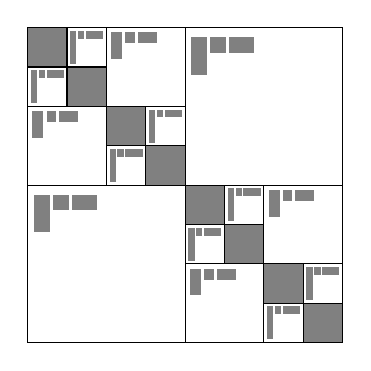
\begin{tikzpicture}[scale=4]
      \path[use as bounding box] (0,0) rectangle (1,1); % adjust to fit
      \draw (0,0) rectangle (1,1);
      \draw (0,0) rectangle (0.5,0.5);
      \draw (1,1) rectangle (0.5,0.5);
      \draw (0,1) rectangle (0.25,0.75);
      \draw [fill=gray] (0,1) rectangle (0.25/2,0.75+0.25/2);
      \draw [fill=gray] (0.25/2,0.75+0.25/2) rectangle (0.25,0.75);
      \draw (0.5,0.5) rectangle (0.75,0.25);
      \draw [fill=gray] (0.5,0.5) rectangle (0.75-0.25/2,0.25+0.25/2);
      \draw [fill=gray] (0.75-0.25/2,0.25+0.25/2) rectangle (0.75,0.25);
      \draw (0.25,0.75) rectangle (0.5,0.5);
      \draw [fill=gray] (0.25,0.75) rectangle (0.5-0.25/2,0.5+0.25/2);
      \draw [fill=gray] (0.5-0.25/2,0.5+0.25/2) rectangle (0.5,0.5);
      \draw (0.75,0.25) rectangle (1,0);
      \draw [fill=gray] (0.75,0.25) rectangle (0.75+0.25/2,0.25/2);
      \draw [fill=gray] (0.75+0.25/2,0.25/2) rectangle (1,0);

      \path [fill=gray] (0.02,0.35) rectangle (0.07,0.47);
      \path [fill=gray] (0.08,0.42) rectangle (0.13,0.47);
      \path [fill=gray] (0.14,0.42) rectangle (0.22,0.47);

      \path [fill=gray] (0.02+0.5,0.35+0.5) rectangle (0.07+0.5,0.47+0.5);
      \path [fill=gray] (0.08+0.5,0.42+0.5) rectangle (0.13+0.5,0.47+0.5);
      \path [fill=gray] (0.14+0.5,0.42+0.5) rectangle (0.22+0.5,0.47+0.5);

      \path [fill=gray] (0.25+0.01+0.5,0.01) rectangle (0.25+0.03+0.5,0.25/2-0.01);
      \path [fill=gray] (0.25+0.035+0.5,0.25/2-0.025-0.01) rectangle (0.25+0.055+0.5,0.25/2-0.01);
      \path [fill=gray] (0.25+0.06+0.5,0.25/2-0.025-0.01) rectangle (0.25+0.25/2-0.01+0.5,0.25/2-0.01);
      \path [fill=gray] (0.25/2+0.25+0.01+0.5,0.25/2+0.01) rectangle (0.25/2+0.25+0.03+0.5,0.25/2+0.25/2-0.01);
      \path [fill=gray] (0.25/2+0.25+0.035+0.5,0.25/2+0.25/2-0.025-0.01) rectangle (0.25/2+0.25+0.055+0.5,0.25/2+0.25/2-0.01);
      \path [fill=gray] (0.25/2+0.25+0.06+0.5,0.25/2+0.25/2-0.025-0.01) rectangle (0.25/2+0.25+0.25/2-0.01+0.5,0.25/2+0.25/2-0.01);
      \path [fill=gray] (0.01+0.5,0.01+0.25) rectangle (0.03+0.5,0.25/2-0.01+0.25);
      \path [fill=gray] (0.035+0.5,0.25/2-0.025-0.01+0.25) rectangle (0.055+0.5,0.25/2-0.01+0.25);
      \path [fill=gray] (0.06+0.5,0.25/2-0.025-0.01+0.25) rectangle (0.25/2-0.01+0.5,0.25/2-0.01+0.25);
      \path [fill=gray] (0.25/2+0.01+0.5,0.25/2+0.01+0.25) rectangle (0.25/2+0.03+0.5,0.25/2+0.25/2-0.01+0.25);
      \path [fill=gray] (0.25/2+0.035+0.5,0.25/2+0.25/2-0.025-0.01+0.25) rectangle (0.25/2+0.055+0.5,0.25/2+0.25/2-0.01+0.25);
      \path [fill=gray] (0.25/2+0.06+0.5,0.25/2+0.25/2-0.025-0.01+0.25) rectangle (0.25/2+0.25/2-0.01+0.5,0.25/2+0.25/2-0.01+0.25);

      \path [fill=gray] (-0.5+0.25+0.01+0.5,0.5+0.01) rectangle (-0.5+0.25+0.03+0.5,0.5+0.25/2-0.01);
      \path [fill=gray] (-0.5+0.25+0.035+0.5,0.5+0.25/2-0.025-0.01) rectangle (-0.5+0.25+0.055+0.5,0.5+0.25/2-0.01);
      \path [fill=gray] (-0.5+0.25+0.06+0.5,0.5+0.25/2-0.025-0.01) rectangle (-0.5+0.25+0.25/2-0.01+0.5,0.5+0.25/2-0.01);
      \path [fill=gray] (-0.5+0.25/2+0.25+0.01+0.5,0.5+0.25/2+0.01) rectangle (-0.5+0.25/2+0.25+0.03+0.5,0.5+0.25/2+0.25/2-0.01);
      \path [fill=gray] (-0.5+0.25/2+0.25+0.035+0.5,0.5+0.25/2+0.25/2-0.025-0.01) rectangle (-0.5+0.25/2+0.25+0.055+0.5,0.5+0.25/2+0.25/2-0.01);
      \path [fill=gray] (-0.5+0.25/2+0.25+0.06+0.5,0.5+0.25/2+0.25/2-0.025-0.01) rectangle (-0.5+0.25/2+0.25+0.25/2-0.01+0.5,0.5+0.25/2+0.25/2-0.01);
      \path [fill=gray] (-0.5+0.01+0.5,0.5+0.01+0.25) rectangle (-0.5+0.03+0.5,0.5+0.25/2-0.01+0.25);
      \path [fill=gray] (-0.5+0.035+0.5,0.5+0.25/2-0.025-0.01+0.25) rectangle (-0.5+0.055+0.5,0.5+0.25/2-0.01+0.25);
      \path [fill=gray] (-0.5+0.06+0.5,0.5+0.25/2-0.025-0.01+0.25) rectangle (-0.5+0.25/2-0.01+0.5,0.5+0.25/2-0.01+0.25);
      \path [fill=gray] (-0.5+0.25/2+0.01+0.5,0.5+0.25/2+0.01+0.25) rectangle (-0.5+0.25/2+0.03+0.5,0.5+0.25/2+0.25/2-0.01+0.25);
      \path [fill=gray] (-0.5+0.25/2+0.035+0.5,0.5+0.25/2+0.25/2-0.025-0.01+0.25) rectangle (-0.5+0.25/2+0.055+0.5,0.5+0.25/2+0.25/2-0.01+0.25);
      \path [fill=gray] (-0.5+0.25/2+0.06+0.5,0.5+0.25/2+0.25/2-0.025-0.01+0.25) rectangle (-0.5+0.25/2+0.25/2-0.01+0.5,0.5+0.25/2+0.25/2-0.01+0.25);

      \path [fill=gray] (0.015,0.15+0.5) rectangle (0.05,0.235+0.5);
      \path [fill=gray] (0.06,0.2+0.5) rectangle (0.09,0.235+0.5);
      \path [fill=gray] (0.1,0.2+0.5) rectangle (0.16,0.235+0.5);
      \path [fill=gray] (0.015+0.25,0.15+0.75) rectangle (0.05+0.25,0.235+0.5+0.25);
      \path [fill=gray] (0.06+0.25,0.2+0.75) rectangle (0.09+0.25,0.235+0.5+0.25);
      \path [fill=gray] (0.1+0.25,0.2+0.75) rectangle (0.16+0.25,0.235+0.5+0.25);

      \path [fill=gray] (0.5+0.015,0.15+0.5-0.5) rectangle (0.5+0.05,0.235+0.5-0.5);
      \path [fill=gray] (0.5+0.06,0.2+0.5-0.5) rectangle (0.5+0.09,0.235+0.5-0.5);
      \path [fill=gray] (0.5+0.1,0.2+0.5-0.5) rectangle (0.5+0.16,0.235+0.5-0.5);
      \path [fill=gray] (0.5+0.015+0.25,0.15+0.75-0.5) rectangle (0.5+0.05+0.25,0.235+0.5+0.25-0.5);
      \path [fill=gray] (0.5+0.06+0.25,0.2+0.75-0.5) rectangle (0.5+0.09+0.25,0.235+0.5+0.25-0.5);
      \path [fill=gray] (0.5+0.1+0.25,0.2+0.75-0.5) rectangle (0.5+0.16+0.25,0.235+0.5+0.25-0.5);
    \end{tikzpicture}
    \vspace{-4mm}
  \end{center}
  \caption{Illustration of a Hierarchically Semi-Separable (HSS)
    matrix. Gray blocks are dense matrices. Off-diagonal blocks, on
    different levels of the HSS hierarchy, are low-rank. The low-rank
    factors of off-diagonal blocks of different levels are related.}
  \label{fig:hss_matrix}
\end{figure}

The sparse multifrontal solver can optionally use Hierarchically
Semi-Separable, rank-structured matrices to compress the fill-in. In
the multifrontal method, computations are performed on dense matrices
called frontal matrices. A frontal matrix can be approximated as an
HSS matrix, but this will only be beneficial (compared to storing the
frontal as a standard dense matrix and operating on it with
BLAS/LAPACK routines) if the frontal matrix is large enough.

Figure~\ref{fig:hss_matrix} illustrates the HSS matrix format. The
matrix is partitioned as a 2 $\times$ 2 block matrix, with the
partitioning recursively applied on the diagonal blocks, until
diagonal blocks are smaller than a specified \emph{leaf size}. The
off-diagonal block on each level of the hierarchy are approximated by
a low-rank product. This low-rank storage format asymptotically
reduces memory usage and floating point operations, while introducing
approximation errors. HSS compression is not used by default in the
STRUMPACK sparse solver (the default is to perform exact LU
factorization), but can be turned on/off via the command line:
\begin{lstlisting}[style=Bash]
  --sp_enable_hss   (no argument)
  --sp_disable_hss   (no argument)
\end{lstlisting}
or via the C\texttt{++} API as follows
\begin{lstlisting}[style=C]
  void SPOptions<scalar>::enable_HSS();
  void SPOptions<scalar>::disable_HSS();
  bool SPOptions<scalar>::use_HSS();    // check whether HSS compression is enabled
\end{lstlisting}
When HSS compression is enabled, the default STRUMPACK behavior is to
use the HSS enabled approximate LU factorization as a preconditioner
within GMRES. This behavior can also be changed, see
Section~\ref{subsec:use_solve}.

However, HSS compression has a considerable overhead and only pays off
for sufficiently large matrices. Therefore STRUMPACK has a tuning
parameter to specify the minimum size a dense matrix needs to be to be
considered a candidate for HSS compression. The minimum dense matrix
size for HSS compression is set via the command line via
\begin{lstlisting}[style=Bash]
  --sp_hss_min_sep_size int (default 256)
\end{lstlisting}
% --sp_hss_min_front_size int (default 1000)
or via the C\texttt{++} API as follows
\begin{lstlisting}[style=C]
  void SPOptions<scalar>::set_HSS_min_sep_size(int s);
  int SPOptions<scalar>::HSS_min_sep_size() const;   // get the current value
\end{lstlisting}
%  void SPOptions<scalar>::set_HSS_min_front_size(int s);
%  int SPOptions<scalar>::HSS_min_front_size() const;
The routine % \lstinline[style=C]!set_HSS_min_front_size(int s)! sets
% the minimum size of the entire front, while
\lstinline[style=C]!set_HSS_min_sep_size(int s)! refers to the size of
the top-left block of the front only. This top-left block is the part
that corresponds to a separator, as given by the nested dissection
reordering algorithm. This top-left block is also referred to as the
block containing the fully-summed variable. Factorization (LU in the
dense case, ULV in the HSS case) is only applied to this top-left
block.
% \emph{\textbf{Tuning the values for the minimum front and separator
% sizes can have a big impact on performance and memory usage!}}
\emph{\textbf{Tuning the value for the minimum separator size can have
    a big impact on performance and memory usage!}}

The above options affect the use of HSS within the multifrontal
solver. There are more, HSS specific, options which are stored in an
object of type \lstinline[style=C]!HSS::HSSOptions<scalar>!. An object
of this type is stored in the \lstinline[style=C]!SPOptions<scalar>!
object stored in the \lstinline[style=C]!StrumpackSparseSolver!. It
can be accessed via the \lstinline[style=C]!HSS_options()! routine as
follows:
\begin{lstlisting}[style=C]
  StrumpackSparseSolver<double> sp;               // create solver object
  sp.options().enable_HSS();                      // enable HSS compression in the multifrontal solver
  sp.options().HSS_options().set_leaf_size(256);  // set the HSS leaf size
\end{lstlisting}

In STRUMPACK, HSS matrices are constructed using a randomized sampling
algorithm~\cite{martinsson2011fast}. To construct an HSS approximation
for a matrix $A$, sampling of the rows and columns of $A$ is computed
by multiplication with a tall and skinny random matrix $R$ as follows:
$S^r = A R$ and $S^c = A^* R$. Ideally, the number of columns in the
matrix $R$ is $d = r + p$, with $r$ the maximum off-diagonal block
rank in the HSS matrix and $p$ a small oversampling
parameter. Unfortunately, the HSS rank is not known a-priori, so it
needs to determined adaptively. The adaptive sampling scheme used in
STRUMPACK starts with an initial number of random vector $d_0$, and
increases this in steps of $\Delta d$, until the compression quality
reaches the desired user specified tolerance, or until the maximum
rank is reached. \emph{\textbf{The compression tolerances can greatly
    impact performance.}} They can be set using:
\begin{lstlisting}[style=Bash]
  --hss_rel_tol real (default 0.01)
  --hss_abs_tol real (default 1e-08)
\end{lstlisting}
or via the C\texttt{++} API
\begin{lstlisting}[style=C]
  void HSSOptions<scalar>::set_rel_tol(real rel_tol);
  void HSSOptions<scalar>::set_abs_tol(real abs_tol);
  real HSSOptions<scalar>::rel_tol() const;    // get the current value
  real HSSOptions<scalar>::abs_tol() const;
\end{lstlisting}

\subsection{\lstinline[style=C]!HSSOptions<scalar>! Interface}
Other options are available to tune for instance the initial number of
random vectors $d_0$, the increment $\Delta d$, the random number
generator or the random number distribution. The complete public
interface for the \lstinline[style=C]!HSSOptions<scalar>! class is:
\begin{lstlisting}[style=C]
  template<typename scalar> class HSSOptions {
  public:
    /* relative compression tolerance                       */
    void set_rel_tol(real rel_tol);           real rel_tol() const;
    /* absolute compression tolerance                       */
    void set_abs_tol(real abs_tol);           real abs_tol() const;
    /* size of the smallest blocks in the HSS hierarchy     */
    void set_leaf_size(int leaf_size);        int leaf_size() const;
    /* initial number of random vectors used in the
       adaptive randomized compression algorithm            */
    void set_d0(int d0);                      int d0() const;
    /* number of random vectors added in each step of the
       adaptive randomized HSS compression algorithm        */
    void set_dd(int dd);                      int dd() const;
    /* currently not used                                   */
    void set_q(int q);                        int q() const;
    /* maximum rank in the HSS representation               */
    void set_max_rank(int max_rank);          int max_rank() const;
    /* random engine/generator to use, see below            */
    void set_random_engine(random::RandomEngine random_engine);
    random::RandomEngine random_engine() const;
    /* the random number distribution, see below            */
    void set_random_distribution
    (random::RandomDistribution random_distribution);
    random::RandomDistribution random_distribution() const;
    /* the compression algorithm to use                     */
    void set_compression_algorithm(CompressionAlgorithm a);
    CompressionAlgorithm compression_algorithm() const;
    /* for expert users                                     */
    void set_user_defined_random(bool user_defined_random);
    bool user_defined_random() const;
    /* for expert users                                     */
    void set_synchronized_compression(bool sync);
    bool synchronized_compression() const;
    /* currently not used                                   */
    void set_log_ranks(bool log_ranks);       bool log_ranks() const;
    /* print statistics?                                    */
    void set_verbose(bool verbose);           bool verbose() const;

    /* parse options in argc/argv                           */
    void set_from_command_line(int argc, char* argv[]);
    /* print description of command line options            */
    void describe_options() const;
  };
\end{lstlisting}

\subsection{HSS Command Line Options}
The HSS specific command line options are:
\begin{lstlisting}[style=Bash]
 HSS Options:
   --hss_rel_tol real (default 0.01)
   --hss_abs_tol real (default 1e-08)
   --hss_leaf_size int (default 128)
   --hss_d0 int (default 128)
   --hss_dd int (default 32)
   --hss_q int (default 0)
   --hss_max_rank int (default 5000)
   --hss_random_distribution normal|uniform (default normal(0,1))
   --hss_random_engine linear|mersenne (default minstd_rand)
   --hss_compression_algorithm original|stable (default stable)
   --hss_user_defined_random (default false)
   --hss_enable_sync (default true)
   --hss_disable_sync (default false)
   --hss_log_ranks (default false)
   --hss_verbose or -v (default false)
   --hss_quiet or -q (default true)
   --help or -h
\end{lstlisting}

\section{HSS Approximation of Dense Matrices}
The HSS code can be found in the \lstinline[style=Bash]!src/HSS/!
subdirectory. All HSS code is in a namespace called
\lstinline[style=C]!HSS!. The class for a sequential/multithreaded HSS
matrix is \lstinline[style=C]!HSSMatrix<scalar>!, while the
distributed memory HSS class is
\lstinline[style=C]!HSSMatrix<scalar>!. For examples of the usage of
these classes, see the test code in
\lstinline[style=Bash]!test/test_HSS_seq.cpp! and
\lstinline[style=Bash]!test/test_HSS_mpi.cpp! respectively. There is
also one sequential example in
\lstinline[style=Bash]!examples/MLkernel.cpp!, which uses HSS
compression for kernel matrices as used in certain machine learning
applications, see for instance~\cite{BirosNlogN}. This part of the
code will be better documented in future STRUMPACK releases.


\section{Examples}\label{sec:examples}
A number of examples are available in the
\lstinline[style=Bash]!examples/! folder. This folder, with the
sources, is copied to the build directory when running
\lstinline[style=Bash]!cmake!. However, the examples are not part of
the CMake build system, so they will not be compiled and linked when
running \lstinline[style=Bash]!make!. A simple
\lstinline[style=Bash]!Makefile! is generated in the
\lstinline[style=Bash]!examples/! folder in the build directory, with
the compiler setting based on what CMake has discovered. However, this
Makefile is rather simplistic and in certain cases it might need some
manual edits. However, it can serve as an example for how to compile
code using STRUMPACK. Check the README file in the
\lstinline[style=Bash]!examples/! directory for more details.

% \todo[inline]{TODO refer to examples folder with examples of:}
% \todo[inline]{Explain how to build the examples!!!}
% \begin{itemize}
% \item Factor once, solve multiple times
% \item Reorder, factor solve, change matrix values but reuse reordering!
% \item A complex arithmetic example
% \item A single precision factorization and a double precision solve??
% \end{itemize}

\section{C Interface} \label{sec:Cinterface} The C interface is
defined in the header file
\lstinline[style=C]!StrumpackSparseSolver.h! and is very similar to
the C\texttt{++} interface. For example usage see the programs
\lstinline[style=C]!sexample.c!, \lstinline[style=C]!dexample.c!,
\lstinline[style=C]!cexample.c! and \lstinline[style=C]!zexample.c!
in the \lstinline[style=C]!examples/! directory, for simple single and
double precision real and complex example programs. Note that since
the STRUMPACK code is written in C\texttt{++}, even when using the C
interface you should link with a C\texttt{++} aware linker or link
with the standard C\texttt{++} library. For instance when using the
GNU toolchain, link with \texttt{g++} instead of \texttt{gcc} or link
with \texttt{gcc} and include \texttt{-lstdc++}.


\section{Advanced Usage Tips}\label{sec:tips}
\begin{itemize}
% \item It is recommended to link with the \texttt{TCMalloc} library
%   (\lstinline[style=Bash]!-ltcmalloc!). \texttt{TCMalloc} replaces the
%   default memory allocator (C\texttt{++} \texttt{new}) with a more
%   scalable implementation. Alternatively, you can link with the
%   Intel\tm{} TBB Scalable Allocator
%   (\lstinline[style=Bash]!-ltbbmalloc!), in which case you also need
%   to configure with \lstinline[style=Bash]!-DCMAKE_CXX_FLAGS="-DUSE_TBB_MALLOC"!.
\item To keep track of the number of floating point operations
  performed in the STRUMPACK Sparse Solver, you can run CMake with
  \lstinline[style=Bash]!-DSTRUMPACK_COUNT_FLOPS=ON!. Then, when
  running, do not set the \texttt{quiet} flag in the
  StrumpackSparseSolver constructor or on the command line and the
  solver will print some statistics. This will also enable a counter
  for data movement in the solve phase, from which the (approximately)
  attained bandwidth usage is derived. This is done because the solve
  phase is typically bandwidth limited, while the factorization is
  flop limited.
\item There is also some support for PAPI. Run CMake with
  \lstinline[style=Bash]!-DSTRUMPACK_USE_PAPI=ON! and specify the PAPI
  include folders and libraries via
  \lstinline[style=Bash]!-DPAPI_INCLUDES=..! and
  \lstinline[style=Bash]!-DPAPI_LIBRARIES=..!.
\item We have added timers all throughout the code. These can be
  enabled with
  \lstinline[style=Bash]!-DSTRUMPACK_TASK_TIMERS=ON!. Running the code
  will generate a file \lstinline[style=Bash]!time.log!. A script to
  visualize these timings is provided.
\item If you compile with MKL or OpenBLAS, you can take advantage of
  some extra optimized routines by specifying
  \lstinline[style=Bash]!-D__HAVE_MKL!  or
  \lstinline[style=Bash]!-D__HAVE_OPENBLAS! respectively.
\item The code is not completely thread safe at the moment: do not
  call solve on the same \lstinline[style=C]!StrumpackSparseSolve!
  object from different threads simultaneously.
\item For comments, feature requests or bug reports:
  \texttt{\{pghysels,xsli,gichavez\}@lbl.gov}
\end{itemize}


\section{FAQ}

\begin{itemize}
\item Help, I get this compilation error:\\
  \verb!catastrophic error: cannot open source file "chrono"! \\
  \verb!#include <chrono>!

  You need a C\texttt{++}11 capable compiler, and also a
  \textbf{C\texttt{++}11 enabled standard library}. For instance
  suppose you are using the Intel 15.0 C\texttt{++} compiler with GCC
  4.4 headers. The Intel 15.0 C\texttt{++} compiler supports the
  C\texttt{++}11 standard, but the GCC 4.4 headers do not implement
  the C\texttt{++}11 standard library. You should install/load a newer
  GCC version (or just the headers). On cray machines, this can be
  done with \lstinline[style=Bash]!module unload gcc; module load gcc/4.9.3!
  for instance.

\item When running \lstinline[style=Bash]!make test!, many of the
  tests fail!

  The parallel execution in ctest is invoked by the
  \lstinline[style=Bash]!MPIEXEC! command as discovered by CMake. On
  many HPC clusters, this does not run unless it is executed from
  within a batch script. In this case all parallel tests will fail. At
  the moment, a small number of tests still fail. This is normal
  behavior.
\end{itemize}


\section{Acknowledgements}
The new, more robust version of the adaptive randomized HSS
compression algorithm was developed in collaboration with Theo Mary
from the Universit\'e de Toulouse.

The code for the STRUMPACK-sparse is based on the sequential code
StruMF, originally developed by Artem Napov. We wish to thank people
who sent us test problems and helped testing the code: Alex Druinsky,
Yvan Notay and Shen Wang.

Partial support for this work was provided through Scientific
Discovery through Advanced Computing (SciDAC) program funded by
U.S. Department of Energy, Office of Science, Advanced Scientific
Computing Research (and Basic Energy Sciences/Biological and
Environmental Research/High Energy Physics/Fusion Energy
Sciences/Nuclear Physics). This research was supported by the Exascale
Computing Project (17-SC-20-SC), a collaborative effort of the
U.S. Department of Energy Office of Science and the National Nuclear
Security Administration.


\section{Copyright notice}
STRUMPACK -- STRUctured Matrices PACKage, Copyright (c) 2014, The
Regents of the University of California, through Lawrence Berkeley
National Laboratory (subject to receipt of any required approvals from
the U.S. Dept. of Energy). All rights reserved.\\

If you have questions about your rights to use or distribute this
software, please contact Berkeley Lab's Technology Transfer Department
at TTD@lbl.gov.\\

NOTICE. This software is owned by the U.S. Department of Energy. As
such, the U.S. Government has been granted for itself and others
acting on its behalf a paid-up, nonexclusive, irrevocable, worldwide
license in the Software to reproduce, prepare derivative works, and
perform publicly and display publicly. Beginning five (5) years after
the date permission to assert copyright is obtained from the
U.S. Department of Energy, and subject to any subsequent five (5) year
renewals, the U.S. Government is granted for itself and others acting
on its behalf a paid-up, nonexclusive, irrevocable, worldwide license
in the Software to reproduce, prepare derivative works, distribute
copies to the public, perform publicly and display publicly, and to
permit others to do so.

\section{License agreement}
"STRUMPACK -- STRUctured Matrices PACKage, Copyright (c) 2014, The
Regents of the University of California, through Lawrence Berkeley
National Laboratory (subject to receipt of any required approvals
from the U.S. Dept. of Energy).  All rights reserved."\\

Redistribution and use in source and binary forms, with or without
modification, are permitted provided that the following conditions
are met:

\begin{enumerate}
\item Redistributions of source code must retain the above copyright
  notice, this list of conditions and the following disclaimer.

\item Redistributions in binary form must reproduce the above
  copyright notice, this list of conditions and the following
  disclaimer in the documentation and/or other materials provided with
  the distribution.

\item Neither the name of the University of California, Lawrence
  Berkeley National Laboratory, U.S. Dept. of Energy nor the names of
  its contributors may be used to endorse or promote products derived
  from this software without specific prior written permission.
\end{enumerate}

THIS SOFTWARE IS PROVIDED BY THE COPYRIGHT HOLDERS AND CONTRIBUTORS
"AS IS" AND ANY EXPRESS OR IMPLIED WARRANTIES, INCLUDING, BUT NOT
LIMITED TO, THE IMPLIED WARRANTIES OF MERCHANTABILITY AND FITNESS
FOR A PARTICULAR PURPOSE ARE DISCLAIMED. IN NO EVENT SHALL THE
COPYRIGHT OWNER OR CONTRIBUTORS BE LIABLE FOR ANY DIRECT, INDIRECT,
INCIDENTAL, SPECIAL, EXEMPLARY, OR CONSEQUENTIAL DAMAGES (INCLUDING,
BUT NOT LIMITED TO, PROCUREMENT OF SUBSTITUTE GOODS OR SERVICES;
LOSS OF USE, DATA, OR PROFITS; OR BUSINESS INTERRUPTION) HOWEVER
CAUSED AND ON ANY THEORY OF LIABILITY, WHETHER IN CONTRACT, STRICT
LIABILITY, OR TORT (INCLUDING NEGLIGENCE OR OTHERWISE) ARISING IN
ANY WAY OUT OF THE USE OF THIS SOFTWARE, EVEN IF ADVISED OF THE
POSSIBILITY OF SUCH DAMAGE.\\

You are under no obligation whatsoever to provide any bug fixes,
patches, or upgrades to the features, functionality or performance
of the source code ("Enhancements") to anyone; however, if you
choose to make your Enhancements available either publicly, or
directly to Lawrence Berkeley National Laboratory, without imposing
a separate written license agreement for such Enhancements, then you
hereby grant the following license: a non-exclusive, royalty-free
perpetual license to install, use, modify, prepare derivative works,
incorporate into other computer software, distribute, and sublicense
such enhancements or derivative works thereof, in binary and source
code form.


\bibliography{\jobname}

\begin{filecontents}{\jobname.bib}
@book{blackford1997scalapack,
  title={ScaLAPACK users' guide},
  author={Blackford, L Susan and Choi, Jaeyoung and Cleary, Andy and D'Azevedo, Eduardo and Demmel, James W and Dhillon, Inderjit and Dongarra, Jack J and Hammarling, Sven and Henry, Greg and Petitet, Antoine and Stanley, Ken and Walker, David and Whaley, R Clinton},
  volume={4},
  year={1997},
  publisher={SIAM},
  url={http://www.netlib.org/scalapack/slug/}
}
@article{martinsson2011fast,
  title={A fast randomized algorithm for computing a hierarchically semiseparable representation of a matrix},
  author={Martinsson, Per-Gunnar},
  journal={SIAM Journal on Matrix Analysis and Applications},
  volume={32},
  number={4},
  pages={1251--1274},
  year={2011},
  publisher={SIAM}
}
@article{rouet2014distributed,
  title={A distributed-memory package for dense Hierarchically Semi-Separable matrix computations using randomization},
  author={Rouet, Fran\c{c}ois-Henry and Li, Xiaoye S. and Ghysels, Pieter},
  journal={ACM Transactions on Mathematical Software},
  year={2016},
  note={to appear}
}
@article{xia2013randomized,
  title={Randomized sparse direct solvers},
  author={Xia, Jianlin},
  journal={SIAM Journal on Matrix Analysis and Applications},
  volume={34},
  number={1},
  pages={197--227},
  year={2013},
  publisher={SIAM}
}
@article{ghysels2015sparse,
  title={An efficient multi-core implementation of a novel {HSS}-structured multifrontal solver using randomized sampling},
  author={Ghysels, Pieter and Li, Xiaoye S. and Rouet, Fran\c{c}ois-Henry and Williams, Samuel and Napov, Artem},
  journal={Submitted to SIAM SISC},
  year={2015}
}
@article{park1993remarks,
  title={Remarks on choosing and implementing random number generators, response (technical correspondence)},
  author={Park, Stephen K and Miller, Keith W and Stockmeyer, Paul K},
  journal={Communications of the ACM},
  volume={36},
  number={7},
  pages={108--110},
  year={1993}
}
@article{matsumoto1998mersenne,
  title={Mersenne twister: a 623-dimensionally equidistributed uniform pseudo-random number generator},
  author={Matsumoto, Makoto and Nishimura, Takuji},
  journal={ACM Transactions on Modeling and Computer Simulation (TOMACS)},
  volume={8},
  number={1},
  pages={3--30},
  year={1998},
  publisher={ACM}
}
@book{saad2003iterative,
  title={{Iterative methods for sparse linear systems}},
  author={Saad, Y.},
  isbn={0898715342},
  year={2003},
  publisher={Society for Industrial Mathematics}
}
@article{duff1999design,
  title={The design and use of algorithms for permuting large entries to the diagonal of sparse matrices},
  author={Duff, Iain S and Koster, Jacko},
  journal={SIAM Journal on Matrix Analysis and Applications},
  volume={20},
  number={4},
  pages={889--901},
  year={1999},
  publisher={SIAM}
}

@INPROCEEDINGS{ghysels2017sparse,
  title={A Robust Parallel Preconditioner for Indefinite Systems Using Hierarchical Matrices and Randomized Sampling},
  author={P. Ghysels and X. S. Li and C. Gorman and F. H. Rouet},
  booktitle={2017 IEEE International Parallel and Distributed Processing Symposium (IPDPS)},
  pages={897-906},
  doi={10.1109/IPDPS.2017.21},
  year={2017},
  month={May},
  publisher={IEEE},
}

@INPROCEEDINGS{BirosNlogN,
  title={{An N log N Parallel Fast Direct Solver for Kernel Matrices}},
  author={D Yu Chenhan, William B March, George Biros},
  booktitle={2017 IEEE International Parallel and Distributed Processing Symposium (IPDPS)},
  pages={886-896},
  doi={10.1109/IPDPS.2017.10},
  year={2017},
  month={May},
  publisher={IEEE},
}

\end{filecontents}

\end{document}

%%% Local Variables:
%%% mode: latex
%%% TeX-master: t
%%% End:
